\chapter{Laboratoriumtechnieken III: onderzoekspraktijk}\label{ch:b3:lab-techniques-3}

Een fles butyllithiumoplossing vat vlam als een druppel met de lucht in
contact komt; een \omterm{def:b3:lab-techniques-3:schlenk}{handschoenkast} houdt zuurstof en water onder enkele ppm,
zodat zulke verbindingen gewogen kunnen worden als keukenzout.
Onderzoekschemie begint vaak met het buitenhouden van de atmosfeer, en
eindigt met een bewering die anderen moeten kunnen controleren: een
nieuwe verbinding, waarvan de structuur en de zuiverheid met meerdere
onafhankelijke methoden bewezen zijn, en waarvan de gegevens vastgelegd
en gepubliceerd zijn zodat het werk herhaald kan worden. Dit laatste
hoofdstuk brengt de onderzoekspraktijk samen: luchtgevoelige stoffen
hanteren, een nieuwe verbinding karakteriseren, een resultaat statistisch
beoordelen, een \omterm{def:b3:lab-techniques-3:notebook}{labjournaal} bijhouden en de literatuur lezen, en de
risico's beoordelen van een procedure die nog niemand uitgevoerd heeft.

\begin{recall}
Het deel van jaar~1 behandelde gevaren, risico's, pictogrammen, H- en
P-zinnen, veiligheidsinformatiebladen en meetonzekerheid met haar
evaluaties van type A en B; het deel van jaar~2 inerte atmosferen,
opwerking, droogmiddelen, flashchromatografie,
massaspectrometrie (HRMS, monoisotopische massa), $^{13}$C-NMR, betrouwbaarheidsintervallen,
de coëfficiënt van Student, ijking, precisie, juistheid, systematische
afwijking, herhaalbaarheid, methodevalidatie, de adiabatische
temperatuurstijging en thermisch op hol slaan.
\Cref{ch:b3:advanced-nmr}, \cref{ch:b3:x-ray-diffraction} en
\cref{ch:b3:electrode-kinetics} leverden de structurele en
elektrochemische methoden.
\end{recall}

\begin{omfigure}
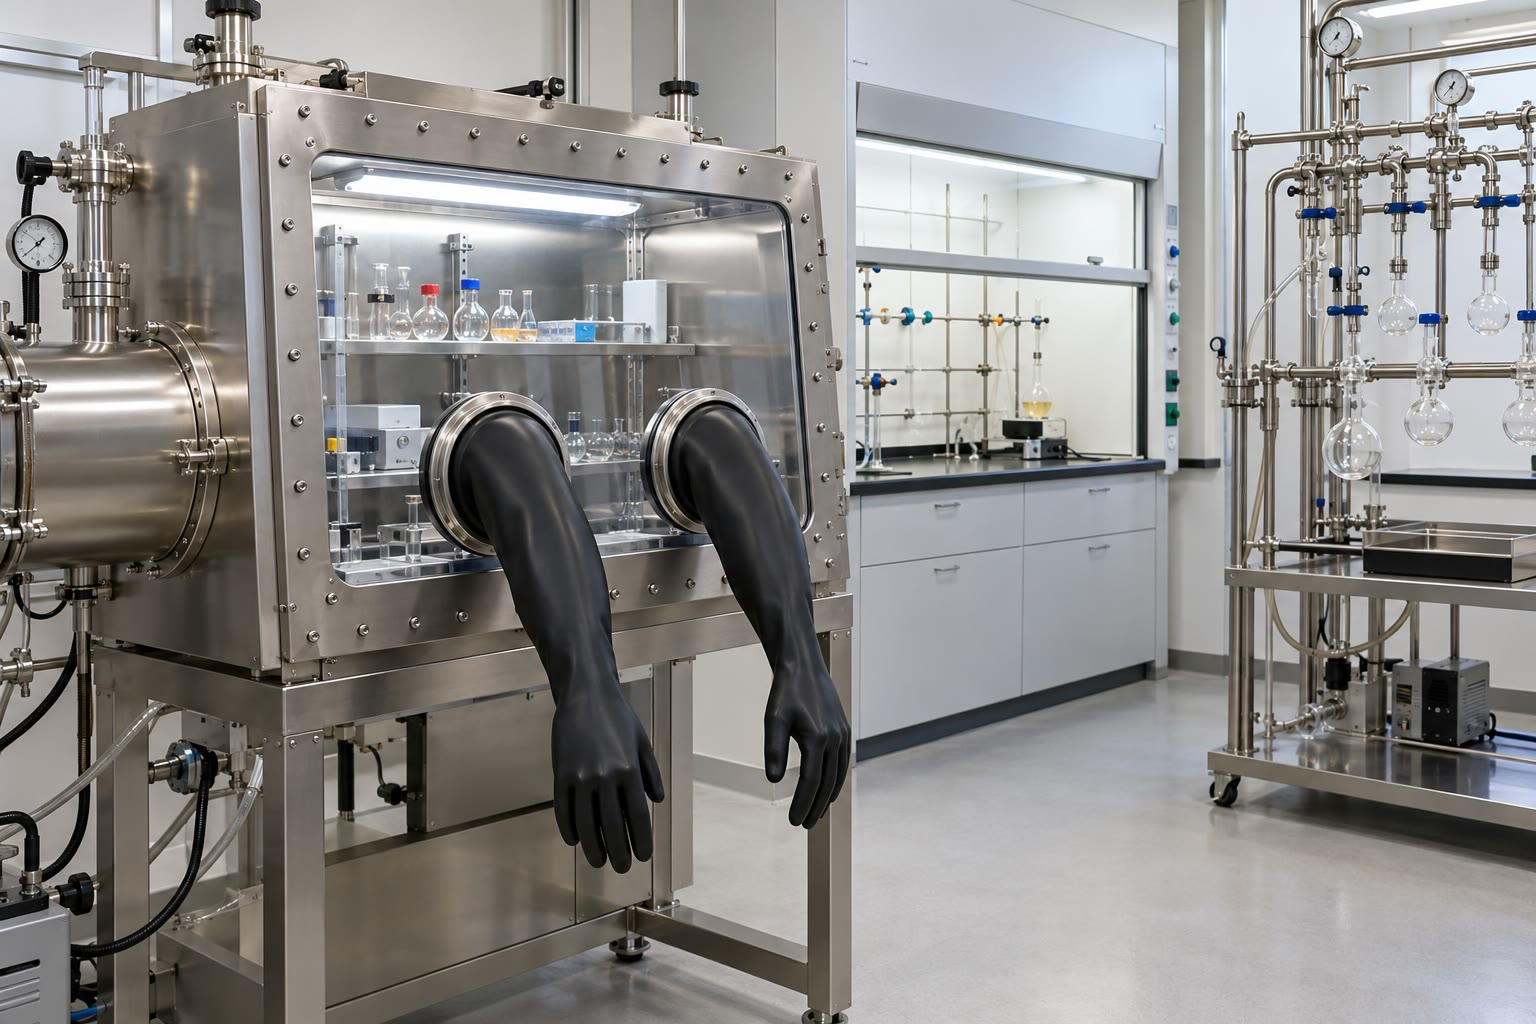
\includegraphics[width=0.58\linewidth]{images/book4/ai/b3-33-glovebox.jpg}

{\small Een onderzoekslaboratorium met een \omterm{def:b3:lab-techniques-3:schlenk}{handschoenkast}: men werkt in de
roestvrijstalen kast, gevuld met droge stikstof of argon, via de
handschoenen; de cilinder links is de sluis om voorwerpen in en uit te
brengen.}
\end{omfigure}

\section{Werken zonder lucht}

\begin{definition}[Luchtgevoelige verbindingen]\label{def:b3:lab-techniques-3:air-sensitive}
Een \emph{luchtgevoelige verbinding}\index{luchtgevoelige verbinding}
reageert met de dizuurstof of het water van de lucht, waarbij ze ontleedt
of haar activiteit verliest. Een
\emph{pyrofore stof}\index{pyrofore stof} ontbrandt spontaan aan de
lucht.
\end{definition}

\begin{definition}[Schlenklijn en handschoenkast]\label{def:b3:lab-techniques-3:schlenk}
Een \emph{schlenklijn}\index{schlenklijn} is een dubbel glazen
verdeelstuk, waarvan de ene buis via een koudeval met een vacuümpomp
verbonden is en de andere met een toevoer van droog inert gas dat via een
olieslot afgevoerd wordt, met kranen die elke uitgang met de ene of de
andere verbinden. Een \emph{schlenkkolf}\index{schlenkkolf} heeft een
zijarm met een kraan om aan de lijn te koppelen. Een
\emph{handschoenkast}\index{handschoenkast} is een gesloten kast gevuld
met inert gas, dat voortdurend gezuiverd wordt, waarin via handschoenen
gewerkt wordt.
\end{definition}

\begin{omfigure}
\begin{tikzpicture}[font=\scriptsize, >=Stealth]
  % manifolds
  \draw[om glass, line width=1.1pt] (0,3.0) -- (8.0,3.0);
  \draw[om glass, line width=1.1pt] (0,2.5) -- (8.0,2.5);
  \node[anchor=east] at (-1.0,3.0) {toevoer van inert gas};
  \node[anchor=east] at (0,2.5) {vacuüm};
  % taps
  \foreach \x in {2.0,4.0,6.0} {
    \draw[om glass] (\x,3.0) -- (\x,2.5);
    \draw[fill=white] (\x,2.75) circle (0.12);
    \draw (\x-0.1,2.75) -- (\x+0.1,2.75);
    \draw[om glass] (\x,2.5) -- (\x,2.0);
  }
  % flask on the middle tap
  \draw[thick, black!60] (4.0,2.0) -- (4.0,1.6) -- (4.6,1.6);
  \pic[scale=0.5, transform shape] at (5.0,-0.2) {rbflask={0.3}{omDef!20}};
  \draw[om glass] (4.6,1.6) -- (4.9,1.25);
  \node[anchor=west] at (5.4,0.4) {schlenkkolf};
  % bubbler at the gas end
  \pic[scale=0.55, transform shape] at (8.9,1.5) {bubbler};
  \draw[om glass] (8.0,3.0) -- (8.6,3.0) -- (8.6,2.9);
  \node[anchor=west] at (9.4,2.2) {olieslot};
  % trap and pump at the vacuum end
  \draw[om glass] (0.4,2.5) -- (0.4,1.6);
  \draw[om glass, fill=omDef!8] (0.15,1.6) rectangle (0.65,0.4);
  \fill[omDef!25] (0.0,0.2) rectangle (0.8,1.2);
  \node[anchor=north] at (0.4,0.2) {koudeval};
  \draw[om glass] (0.65,0.9) -- (1.6,0.9);
  \draw[fill=black!15] (1.6,0.6) rectangle (2.6,1.2);
  \node at (2.1,0.9) {pomp};
  \draw[->, thick] (-0.9,3.0) -- (0,3.0);
\end{tikzpicture}

{\small Een \omterm{def:b3:lab-techniques-3:schlenk}{schlenklijn}, schematisch: een gasverdeelstuk en een
vacuümverdeelstuk, verbonden door kranen; elke kraan verbindt haar kolf
ofwel met het vacuüm ofwel met het inerte gas. Afgepompte
oplosmiddeldamp condenseert in de koudeval voordat hij de pomp bereikt;
het gas vertrekt via een olieslot, dat verhindert dat lucht terugstroomt.}
\end{omfigure}

\begin{proposition}[Cycli van vacuümtrekken en hervullen]\label{prop:b3:lab-techniques-3:purge-cycles}
Als een kolf gevuld met lucht bij druk $p_0$ vacuüm getrokken wordt tot $p_{\min}$ en opnieuw gevuld met
zuiver inert gas, en dat $n$ keer, is de fractie van de oorspronkelijke lucht die overblijft $(p_{\min}/p_0)^n$.
\end{proposition}

\begin{proof}
Vacuüm trekken tot $p_{\min}$ laat een fractie $p_{\min}/p_0$ van het gas achter, met dezelfde samenstelling; het
hervullen met zuiver inert gas herstelt $p_0$ zonder lucht toe te voegen. Elke cyclus vermenigvuldigt de
luchtfractie met $p_{\min}/p_0$; na $n$ cycli is ze $(p_{\min}/p_0)^n$.
\end{proof}

Drie cycli tot \qty{0.1}{mbar} laten op papier $10^{-12}$ van de lucht over; in de praktijk
leggen lekken, gas dat op het glas geadsorbeerd is en het ontgassen van
vet en septa de grens, en daarom wordt glaswerk in een oven gedroogd en
heet gemonteerd.

\begin{definition}[Canuletransfer]\label{def:b3:lab-techniques-3:cannula}
Een \emph{canuletransfer}\index{canuletransfer} brengt een luchtgevoelige
vloeistof van een gesloten vat naar een ander over via een lange naald
met twee punten, aangedreven door een kleine overdruk van inert gas in
het eerste vat.
\end{definition}

\begin{omfigure}
\begin{tikzpicture}[font=\scriptsize, >=Stealth]
  \pic at (0,0) {rbflask={0.35}{omThm!25}};
  \pic at (4.2,0) {rbflask={0.1}{omDef!15}};
  \pic at (0,3.0) {septum};
  \pic at (4.2,3.0) {septum};
  \draw[black!70, line width=0.9pt] (0.05,0.25) -- (0.05,3.5) to[out=90, in=90] (4.15,3.5) -- (4.15,1.6);
  \draw[->, thick, omThm] (1.3,3.95) -- (2.9,3.95) node[midway, above] {vloeistof};
  \draw[->, thick] (-1.3,3.4) -- (-0.15,3.2) node[pos=0, left] {inert gas in (lichte overdruk)};
  \draw[->, thick] (4.35,3.2) -- (5.4,3.6) node[right] {afvoer naar olieslot};
  \node[anchor=north] at (0,-0.1) {bron};
  \node[anchor=north] at (4.2,-0.1) {ontvanger};
\end{tikzpicture}

{\small Een \omterm{def:b3:lab-techniques-3:cannula}{canuletransfer}: de onderste punt van de canule hangt in de
vloeistof van de bronkolf; inert gas dat in de bron gelaten wordt, duwt de
vloeistof door de canule naar de ontvanger, die via een naald naar het
olieslot ontlucht wordt.}
\end{omfigure}

\begin{method}[Een canuletransfer]\label{met:b3:lab-techniques-3:cannula}
\begin{enumerate}
  \item Breng beide kolven, afgesloten met septa, onder inert gas aan de
        \omterm{def:b3:lab-techniques-3:schlenk}{schlenklijn}.
  \item Spoel de canule met gas: steek het ene uiteinde in de bron boven
        de vloeistof tot er gas uit het andere uiteinde stroomt, en steek
        dat uiteinde dan in de ontvanger.
  \item Ontlucht de ontvanger met een naald; duw het bronuiteinde van de
        canule onder het vloeistofoppervlak: de overdruk drijft de
        vloeistof over.
  \item Om te stoppen, til je de punt boven de vloeistof; trek de canule
        eerst uit de ontvanger, en spoel haar meteen in de zuurkast met een
        droog oplosmiddel en daarna met water.
\end{enumerate}
\end{method}

\begin{definition}[Vries-pomp-dooiontgassing]\label{def:b3:lab-techniques-3:degassing}
\emph{Vries-pomp-dooiontgassing}\index{vries-pomp-dooiontgassing}
verwijdert opgeloste gassen uit een vloeistof door haar in vloeibare
stikstof te bevriezen, de ruimte erboven vacuüm te trekken, de kraan te
sluiten en haar te laten ontdooien, zodat het opgeloste gas in het
vacuüm ontsnapt; de cyclus wordt drie keer herhaald.
\end{definition}

Droge oplosmiddelen komen nu uit kolommen met geactiveerd aluminiumoxide
onder inert gas in plaats van uit destillatieopstellingen boven natrium.
Organolithiumoplossingen verliezen met de tijd aan sterkte en worden vóór
gebruik getitreerd, bijvoorbeeld tegen een afgewogen hoeveelheid
difenylazijnzuur in droog THF: het eerste equivalent deprotoneert het
zuur, de eerste druppel overmaat geeft het gele dianion.

\begin{proposition}[Titer van een organolithiumverbinding]\label{prop:b3:lab-techniques-3:titre}
Als een massa $m$ difenylazijnzuur (molaire massa $M$) een volume $V$ van een
organolithiumoplossing nodig heeft om de kleuromslag te bereiken, is de concentratie $c = m/(MV)$.
\end{proposition}

\begin{proof}
Tot het eindpunt neemt elke organolithiumverbinding één proton van het
zuur weg; de kleur verschijnt wanneer het zuur opgebruikt is. De
hoeveelheden zijn gelijk: $cV = m/M$.
\end{proof}

\begin{inthelab}[De sluis van de handschoenkast]
Voorwerpen gaan via de sluis een \omterm{def:b3:lab-techniques-3:schlenk}{handschoenkast} binnen: ze worden erin
geplaatst, de buitendeur wordt gesloten, en de sluis wordt drie keer
vacuüm getrokken en hervuld met het gas van de kast, met een lange
laatste vacuümcyclus voor poreuze voorwerpen, die lucht vasthouden; pas
dan wordt de binnendeur vanuit de kast met de handschoenen geopend.
Oplosmiddelen en open houders met vluchtige vloeistoffen worden nooit in
de sluis vacuüm getrokken, en niets wat de zuiveringseenheid zou
vergiftigen (thiolen, gehalogeneerde oplosmiddelen) wordt zonder
toestemming binnenin geopend.
\end{inthelab}

\begin{omfigure}
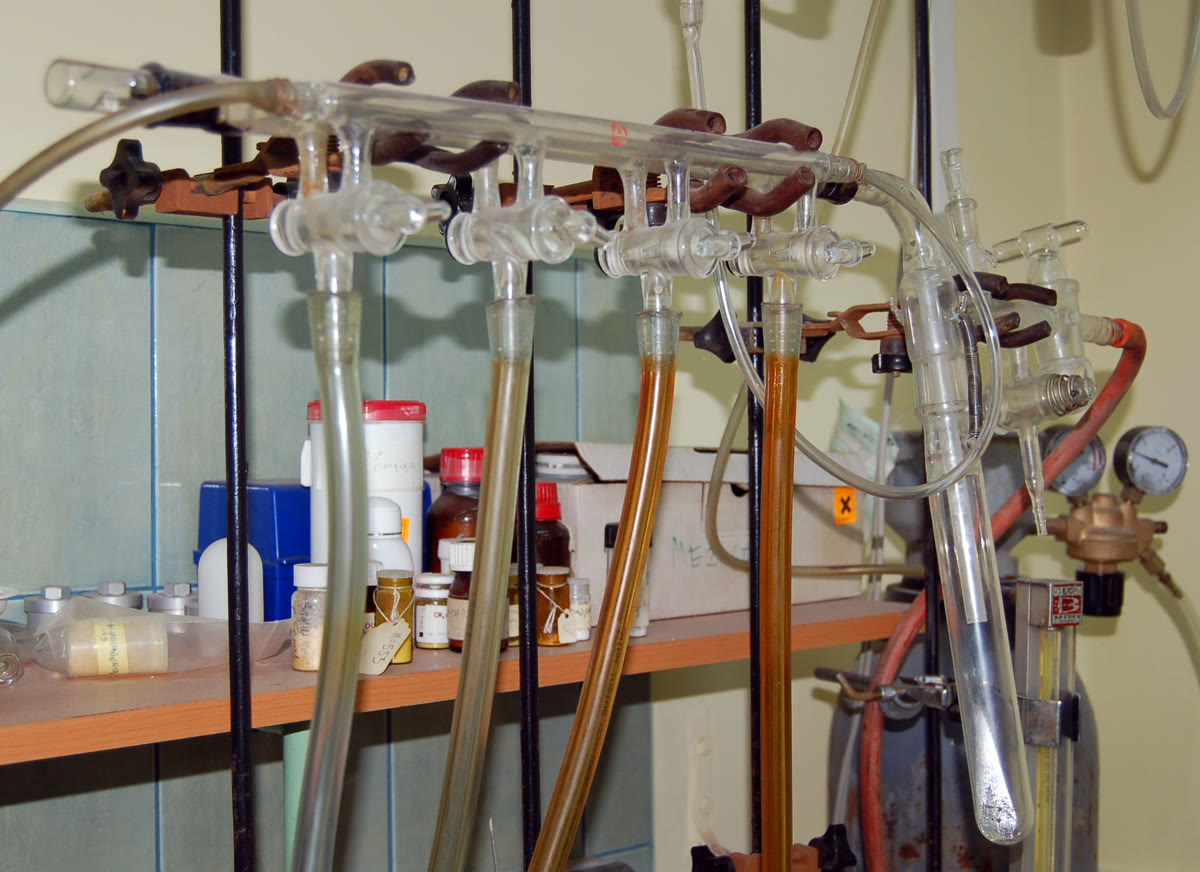
\includegraphics[width=0.46\linewidth]{images/book4/schlenk-line.jpg}

{\small Een \omterm{def:b3:lab-techniques-3:schlenk}{schlenklijn} in gebruik: het glazen verdeelstuk met zijn kranen,
slangen naar de kolven, en de gasregelaar. Foto: Polimerek, CC BY-SA 3.0.}
\end{omfigure}

\section{Een nieuwe verbinding karakteriseren}

\begin{method}[Een nieuwe verbinding karakteriseren]\label{met:b3:lab-techniques-3:characterise}
\begin{enumerate}
  \item Zuiverheid: één vlek in DLC in twee eluentia, één piek in HPLC of
        GC, een scherp smeltpunt; \omterm{def:b3:lab-techniques-3:qnmr}{kwantitatieve NMR} als een
        massazuiverheid nodig is.
  \item Formule: HRMS binnen enkele ppm van de berekende massa, en het
        isotopenpatroon; of \omterm{def:b3:lab-techniques-3:elemental}{elementanalyse}.
  \item Structuur: $^1$H- en $^{13}$C-NMR met 2D-experimenten voor de verbindingen
        (\cref{ch:b3:advanced-nmr}), IR voor de functionele groepen; een
        röntgenstructuur van een éénkristal als er kristallen groeien
        (\cref{ch:b3:x-ray-diffraction}).
  \item Stereochemie: NOE, koppelingsconstanten, optische draaiing, ee
        met chirale chromatografie.
  \item Rapporteer elk gegeven met zijn omstandigheden, en de spectra in
        de \omterm{def:b3:lab-techniques-3:literature}{ondersteunende informatie}.
\end{enumerate}
\end{method}

\begin{omfigure}
\begin{tikzpicture}[font=\scriptsize, >=Stealth,
  box/.style={draw, rounded corners, align=center, fill=omDef!8, inner sep=3pt, minimum height=8mm}]
  \node[box] (a) at (0,0) {nieuwe verbinding\\ geïsoleerd};
  \node[box] (b) at (2.85,0) {zuiver?\\ DLC, HPLC, smp.};
  \node[box] (c) at (5.85,0) {formule\\ HRMS, CHN};
  \node[box] (d) at (8.75,0) {structuur\\ NMR (1D, 2D), IR};
  \node[box] (e) at (8.75,-1.6) {röntgen bij kristallen,\\ stereochemie};
  \node[box, fill=omMeth!12] (f) at (5.85,-1.6) {consistent?\\ rapporteer met\\ ruwe gegevens};
  \node[box, fill=omThm!10] (g) at (2.85,-1.6) {opnieuw zuiveren\\ (chromatografie,\\ kristallisatie)};
  \draw[->, thick] (a) -- (b); \draw[->, thick] (b) -- node[above, inner sep=1pt] {ja} (c);
  \draw[->, thick] (c) -- (d); \draw[->, thick] (d) -- (e); \draw[->, thick] (e) -- (f);
  \draw[->, thick] (b) -- node[left] {nee} (g); \draw[->, thick] (g.north west) to[bend left=30] (a.south);
\end{tikzpicture}

{\small Het verloop van de karakterisering van een nieuwe verbinding:
eerst de zuiverheid, dan de formule, dan de structuur; elke bewering
steunt op minstens twee onafhankelijke methoden, en de \omterm{def:b3:lab-techniques-3:notebook}{ruwe gegevens}
gaan mee met het verslag.}
\end{omfigure}

\begin{definition}[Elementanalyse]\label{def:b3:lab-techniques-3:elemental}
\emph{Elementanalyse}\index{elementanalyse} (verbrandingsanalyse) bepaalt
de massapercentages koolstof, waterstof, stikstof en zwavel in een
monster door het in zuurstof te verbranden en het gevormde
koolstofdioxide, water, distikstof en zwaveldioxide te meten.
\end{definition}

\begin{proposition}[Massapercentages uit een formule]\label{prop:b3:lab-techniques-3:mass-fractions}
Voor een formule $\mathrm{C}_a\mathrm{H}_b\mathrm{N}_c\dots$ met molaire massa $M$ is het massapercentage koolstof $100\,aA_r(\mathrm C)/M$, en evenzo
voor de andere elementen.
\end{proposition}

\begin{proof}
Eén mol verbinding, met massa $M$, bevat $a$ mol koolstofatomen, met massa $aA_r(\mathrm C)$;
de verhouding, maal 100, is het massapercentage.
\end{proof}

% ledger: ea:tolerance, hrms:tolerance
De meeste chemietijdschriften vragen als bewijs van de samenstelling
gevonden waarden voor C, H en N binnen 0.4 procentpunt van de berekende,
of een HRMS-meting binnen enkele ppm (5 ppm voor sommige). Een groot
interlaboratoriumonderzoek vond dat zelfs zuivere monsters verrassend
vaak buiten het criterium van 0.4 vallen, een herinnering dat een
criterium geen natuurwet is.

\begin{proposition}[HRMS-fout]\label{prop:b3:lab-techniques-3:ppm-error}
De fout van een gemeten massa $m_{\mathrm{gem}}$ ten opzichte van de berekende $m_{\mathrm{ber}}$ is
$10^6(m_{\mathrm{gem}} - m_{\mathrm{ber}})/m_{\mathrm{ber}}$ ppm; voor een ion wordt $m_{\mathrm{ber}}$ berekend uit monoisotopische massa's min (of plus) de
massa van de weggenomen (of toegevoegde) elektronen.
\end{proposition}

\begin{proof}[Per definitie]
De ppm-fout is het relatieve verschil uitgedrukt in delen per miljoen;
de massa van het ion verschilt van die van de neutrale formule door de
elektronen, elk \qty{5.486e-4}{u}, enkele ppm bij massa's van enkele
honderden.
\end{proof}

\begin{definition}[Kwantitatieve NMR]\label{def:b3:lab-techniques-3:qnmr}
\emph{Kwantitatieve NMR}\index{kwantitatieve NMR} (qNMR) bepaalt
hoeveelheden of zuiverheden uit signaalintegralen, die evenredig zijn met
het aantal kernen wanneer het spectrum opgenomen wordt met volledige
relaxatie tussen de pulsen, ten opzichte van een interne standaard met
bekende zuiverheid die samen met het monster afgewogen wordt.
\end{definition}

\begin{proposition}[Zuiverheid met qNMR]\label{prop:b3:lab-techniques-3:qnmr}
Voor een monster met massa $m_x$, afgewogen met een standaard met massa $m_s$ en zuiverheid $P_s$, met signalen
met integralen $I_x$ en $I_s$ van $N_x$ en $N_s$ protonen, is
\[
  P_x = \frac{I_x}{I_s}\,\frac{N_s}{N_x}\,\frac{M_x}{M_s}\,\frac{m_s}{m_x}\,P_s.
\]
\end{proposition}

\begin{proof}
De integralen zijn evenredig met het aantal protonen: $I_x/I_s = (N_xn_x)/(N_sn_s)$. Met
$n_x = P_xm_x/M_x$ en $n_s = P_sm_s/M_s$ geeft oplossen naar $P_x$ de formule.
\end{proof}

\begin{omfigure}
\begin{tikzpicture}
\begin{axis}[width=0.8\linewidth, height=5.0cm, x dir=reverse, xmin=3.0, xmax=7.0, ymin=-0.05, ymax=1.15, clip=false,
  axis x line=bottom, axis y line=none, xlabel={$\delta$ / ppm}, tick label style={font=\scriptsize}, label style={font=\small}]
\addplot[color=omDef, thick] table[x=ppm, y=y] {figdata/out/bachelor-3-qnmr.dat};
\node[font=\scriptsize, anchor=south] at (axis cs:6.09,0.33) {standaard, ArH (3 H)};
\node[font=\scriptsize, anchor=east] at (axis cs:4.20,0.98) {ferroceen (10 H)};
\node[font=\scriptsize, anchor=west, align=left] at (axis cs:3.72,0.70) {standaard,\\ $\ce{OCH3}$ (9 H)};
\end{axis}
\end{tikzpicture}

{\small Synthetisch protonspectrum van een ferroceenmonster, afgewogen met
1,3,5-trimethoxybenzeen als interne standaard (model: 20.0 mg monster met
een zuiverheid van 98.0\,\%, 15.0 mg standaard). De integralen zijn
evenredig met het aantal protonen maal de hoeveelheid van elke
verbinding; de verhouding van de singulet van ferroceen tot de
aromatische singulet van de standaard geeft de zuiverheid.}
\end{omfigure}

\section{Statistiek van een onderzoeksresultaat}

\begin{definition}[Significantietoetsen]\label{def:b3:lab-techniques-3:tests}
Een \emph{significantietoets}\index{significantietoets} beslist of
gegevens verenigbaar zijn met een
\emph{nulhypothese}\index{nulhypothese}, meestal dat er geen verschil of
geen effect is, bij een gekozen risico om haar ten onrechte te verwerpen
(vaak 5\,\%).
\end{definition}

\begin{theorem}[$t$-toets voor twee steekproeven]\label{thm:b3:lab-techniques-3:t-test}
Voor twee reeksen van $n_1$ en $n_2$ onafhankelijke metingen uit normale
verdelingen met gelijke standaardafwijking, met gemiddelden $\bar x_1$, $\bar x_2$ en gepoolde
standaardafwijking $s_p$, volgt de grootheid $t = (\bar x_1 - \bar x_2)/(s_p\sqrt{1/n_1 + 1/n_2})$ de wet van Student met
$n_1 + n_2 - 2$ vrijheidsgraden als de twee ware gemiddelden gelijk zijn. \admitted
\end{theorem}

\begin{proposition}[$F$-toets]\label{prop:b3:lab-techniques-3:f-test}
Onder dezelfde aannamen volgt de verhouding $F = s_1^2/s_2^2$ van twee steekproefvarianties
de wet van Fisher met $(n_1 - 1, n_2 - 1)$ vrijheidsgraden als de ware varianties gelijk zijn.
\admitted
\end{proposition}

\begin{method}[Is een nieuw rendement beter?]\label{met:b3:lab-techniques-3:compare-means}
\begin{enumerate}
  \item Herhaal beide procedures meerdere keren onder dezelfde
        omstandigheden; noteer elk resultaat.
  \item Vergelijk eerst de spreidingen ($F$-toets); als ze gelijkaardig zijn, pool ze dan:
        $s_p^2 = [(n_1 - 1)s_1^2 + (n_2 - 1)s_2^2]/(n_1 + n_2 - 2)$.
  \item Bereken $t$ en vergelijk $|t|$ met de coëfficiënt van Student voor $n_1 + n_2 - 2$
        vrijheidsgraden bij het gekozen niveau.
  \item Groter: het verschil is significant. Kleiner: de gegevens tonen er
        geen, wat niet bewijst dat er geen is.
\end{enumerate}
\end{method}

Een verdachte waarde wordt nooit geschrapt omdat ze ongelegen komt.
Uitbijtertoetsen signaleren haar, maar de beslissing berust op het
\omterm{def:b3:lab-techniques-3:notebook}{labjournaal}: een genoteerde oorzaak (een weegfout, een verontreinigde
kolf) rechtvaardigt haar verwerping; zonder oorzaak blijft ze behouden,
of wordt het experiment herhaald.

\section{Het labjournaal, onderzoeksgegevens en de literatuur}

\begin{definition}[Labjournaal en ruwe gegevens]\label{def:b3:lab-techniques-3:notebook}
Het \emph{labjournaal}\index{labjournaal} is het gedateerde, doorlopende,
ongewijzigde verslag van de uitgevoerde experimenten, zoals ze uitgevoerd
werden. \emph{Ruwe gegevens}\index{ruwe gegevens} zijn de oorspronkelijke
registraties van metingen (instrumentbestanden, weegbonnen, spectra)
vóór elke verwerking.
\end{definition}

\begin{method}[Een notitie in het labjournaal schrijven]\label{met:b3:lab-techniques-3:notebook}
\begin{enumerate}
  \item Datum, titel, doel, en een verwijzing naar het vorige verwante
        experiment.
  \item Het reactieschema met de hoeveelheden (massa's, volumes, mol,
        equivalenten), de herkomst en de partijen van de reagentia, en de
        \omterm{def:b3:lab-techniques-3:assessment}{risicobeoordeling}.
  \item Wat er gedaan en waargenomen werd, in volgorde en op het moment
        zelf, ook wat misliep; nooit uitgommen, maar doorhalen zodat het
        origineel leesbaar blijft.
  \item Resultaten: rendementen, de namen van de bestanden met \omterm{def:b3:lab-techniques-3:notebook}{ruwe
        gegevens}, en een besluit; onderteken.
\end{enumerate}
\end{method}

\begin{definition}[FAIR-gegevens]\label{def:b3:lab-techniques-3:fair}
% ledger: fair:year
\emph{FAIR-gegevens}\index{FAIR-gegevens} zijn onderzoeksgegevens die
vindbaar, toegankelijk, interoperabel en herbruikbaar zijn (Findable,
Accessible, Interoperable, Reusable): beschreven met rijke metadata en
een persistente identificator, op te halen via standaardprotocollen, in
open formaten, met een duidelijke licentie en herkomst.
\end{definition}

\begin{definition}[Wetenschappelijke integriteit]\label{def:b3:lab-techniques-3:integrity}
\emph{Wetenschappelijke integriteit}\index{wetenschappelijke integriteit}
is het eerlijk en transparant uitvoeren en rapporteren van onderzoek. De
ernstigste schendingen ervan zijn
\emph{fabricage}\index{fabricage} (gegevens verzinnen),
\emph{falsificatie}\index{falsificatie} (gegevens, beelden of procedures
vervalsen) en \emph{plagiaat}\index{plagiaat} (het werk van anderen als
eigen werk voorstellen).
\end{definition}

\begin{definition}[De literatuur]\label{def:b3:lab-techniques-3:literature}
De \emph{primaire literatuur}\index{primaire literatuur} rapporteert
oorspronkelijk onderzoek (artikels, octrooien, proefschriften); de
\emph{secundaire literatuur}\index{secundaire literatuur} bespreekt en
ordent het (overzichtsartikels, handboeken, databanken), en leerboeken
vormen een tertiaire laag.
\emph{Peerreview}\index{peerreview} is de beoordeling van een manuscript
door onafhankelijke deskundigen vóór de publicatie. De
\emph{ondersteunende informatie}\index{ondersteunende informatie} van een
artikel bevat de experimentele details en gegevens die nodig zijn om het
werk te herhalen en te controleren.
\end{definition}

\begin{method}[Een gepubliceerde procedure lezen]\label{met:b3:lab-techniques-3:read-paper}
\begin{enumerate}
  \item Lees het experimentele deel en de \omterm{def:b3:lab-techniques-3:literature}{ondersteunende informatie}, niet
        alleen de samenvatting en het schema.
  \item Controleer de schaal, de concentraties, de temperaturen, de tijden
        en de opwerking; noteer wat ontbreekt.
  \item Toets de karakterisering van de producten aan de methode
        hierboven.
  \item Zoek latere artikels die de procedure gebruikten of corrigeerden;
        voer haar eerst op kleine schaal uit.
\end{enumerate}
\end{method}

Databanken van structuren en reacties indexeren de \omterm{def:b3:lab-techniques-3:literature}{primaire literatuur}
per verbinding en per omzetting, en worden doorzocht door een structuur
of een reactie te tekenen in plaats van met woorden.

\section{Risicobeoordeling van een nieuwe procedure}

\begin{definition}[Risicobeoordeling]\label{def:b3:lab-techniques-3:assessment}
Een \emph{risicobeoordeling}\index{risicobeoordeling} van een procedure
brengt haar gevaren in kaart, schat de waarschijnlijkheid en de ernst van
schade onder de geplande omstandigheden, en legt de beheersmaatregelen
vast die het risico tot een aanvaardbaar niveau terugbrengen. De
\emph{hiërarchie van beheersmaatregelen}\index{hierarchie van beheersmaatregelen@hiërarchie van beheersmaatregelen}
rangschikt ze van meest tot minst doeltreffend: eliminatie, substitutie,
technische maatregelen, organisatorische maatregelen, persoonlijke
beschermingsmiddelen.
\end{definition}

\begin{omfigure}
\begin{tikzpicture}[font=\scriptsize]
  \foreach \i/\lab/\col in {0/eliminatie: het gevaar wegnemen/omMeth!40, 1/substitutie: een minder gevaarlijk reagens/omMeth!28, 2/technisch: zuurkast{,} handschoenkast{,} schermen/omDef!22, 3/organisatorisch: procedures{,} opleiding/omProp!22, 4/persoonlijke beschermingsmiddelen/omThm!22} {
    \pgfmathsetmacro\w{5.4-0.95*\i}
    \fill[\col] ({-\w/2},{-0.75*\i}) -- ({\w/2},{-0.75*\i}) -- ({\w/2-0.475},{-0.75*\i-0.7}) -- ({-\w/2+0.475},{-0.75*\i-0.7}) -- cycle;
    \node[anchor=west] at (3.0,{-0.75*\i-0.35}) {\lab};
    \draw[black!30] ({\w/2-0.2},{-0.75*\i-0.35}) -- (2.95,{-0.75*\i-0.35});
  }
  \node[anchor=east, align=right] at (-2.9,-0.35) {meest\\ doeltreffend};
  \node[anchor=east, align=right] at (-2.9,-3.35) {minst\\ doeltreffend};
  \draw[->, black!50] (-3.3,-0.85) -- (-3.3,-2.85);
\end{tikzpicture}

{\small De \omterm{def:b3:lab-techniques-3:assessment}{hiërarchie van beheersmaatregelen}, als omgekeerde piramide: het
gevaar wegnemen of vervangen beschermt iedereen, altijd;
beschermingsmiddelen beschermen alleen hun drager, en alleen als ze
gedragen worden en intact zijn.}
\end{omfigure}

\begin{definition}[Peroxidevormers]\label{def:b3:lab-techniques-3:peroxide}
Een \emph{peroxidevormer}\index{peroxidevormer} is een verbinding, zoals
diethylether, tetrahydrofuraan of 1,4-dioxaan, die bij bewaring
langzaam explosieve peroxiden vormt met de lucht, vooral na opening en
onder invloed van licht.
\end{definition}

\begin{method}[De risico's van een nieuwe procedure beoordelen]\label{met:b3:lab-techniques-3:risk-assessment}
\begin{enumerate}
  \item Som elke stof op (reagentia, oplosmiddelen, producten,
        bijproducten, vrijkomende gassen) met haar gevaren uit het
        veiligheidsinformatieblad.
  \item Som de handelingen en hun omstandigheden op (verwarming, druk,
        schaal, afbreken van de reactie, afval); schat de vrijkomende
        warmte en de adiabatische temperatuurstijging voordat je
        opschaalt.
  \item Kies voor elk gevaar beheersmaatregelen volgens de hiërarchie;
        plan het optreden in noodgevallen (lekkage, brand, blootstelling)
        en de afvoer van het afval.
  \item Leg het schriftelijk vast, laat het controleren, en herzie het na
        de eerste uitvoering.
\end{enumerate}
\end{method}

\begin{safety}{\ghs[0.62cm]{GHS02}\ghs[0.62cm]{GHS05}\ghs[0.62cm]{GHS07}\ghs[0.62cm]{GHS08}}
% ledger: ghs4:BuLi, ghs4:Et2O, ghs4:THF
Butyllithiumoplossingen: pyrofoor, reageren hevig met water onder vorming
van ontvlambaar gas, veroorzaken ernstige brandwonden; alleen onder inert
gas gehanteerd, met een emmer droog zand bij de hand en geen water in de
buurt. Natriumhydride zet eveneens waterstof vrij met water en vocht, en
wordt gebruikt als dispersie in olie. Diethylether en THF zijn zeer
licht ontvlambare \omterm{def:b3:lab-techniques-3:peroxide}{peroxidevormers}: gedateerd bij opening, op peroxiden
getest vóór destillatie of indamping, en volgens schema afgevoerd.
\end{safety}

\begin{history}[Het glaswerk van Schlenk]
Wilhelm Schlenk, die in de jaren 1910 organoalkaliverbindingen en
radicalen bestudeerde, ontwierp de kolven en technieken waarmee hij ze
zonder lucht kon hanteren; de lijn en de kolf dragen nog steeds zijn
naam. De eerste \omterm{def:b3:lab-techniques-3:schlenk}{handschoenkasten} werden in de jaren 1940 gebouwd voor
radioactieve materialen en al snel overgenomen door chemici die met
\omterm{def:b3:lab-techniques-3:air-sensitive}{luchtgevoelige verbindingen} werkten.
\end{history}

\section{Oefeningen}

\begin{exercise}[$\star$]\label{exo:b3:lab-techniques-3:1}
Een kolf wordt drie keer vacuüm getrokken tot \qty{0.50}{mbar} en met argon hervuld tot \qty{1013}{mbar}. Welke fractie van
de oorspronkelijke lucht blijft in theorie over? Wat beperkt het
resultaat in werkelijkheid?
\end{exercise}

\begin{exercise}[$\star$]\label{exo:b3:lab-techniques-3:2}
Een butyllithiumoplossing heeft een titer van \qty{1.48}{mol/L}. Welk volume moet overgebracht worden om
\qty{20.0}{mmol} te leveren?
\end{exercise}

\begin{exercise}[$\star$]\label{exo:b3:lab-techniques-3:3}
% ledger: mass:C12, mass:H1, mass:Fe56, const4:me.u, hrms:tolerance
Bereken de exacte massa van het ferroceenradicaalkation $\ce{C10H10Fe+}$ uit monoisotopische massa's
($^{12}$C precies 12, $^1$H 1.00782503, $^{56}$Fe 55.93493633, elektron \qty{5.486e-4}{u}), en de fout van een gemeten
waarde 186.0129 in ppm.
\end{exercise}

\begin{exercise}[$\star$]\label{exo:b3:lab-techniques-3:4}
Deel in als primaire, secundaire of tertiaire literatuur: een
overzichtsartikel, een tijdschriftartikel dat een nieuwe synthese
rapporteert, een octrooi, een handboek van fysische constanten, een
proefschrift, een leerboek.
\end{exercise}

\begin{exercise}[$\star\star$]\label{exo:b3:lab-techniques-3:5}
% ledger: ea:tolerance
Bereken de massapercentages C, H en N van cafeïne, $\ce{C8H10N4O2}$, en beslis of de gevonden
waarden C 49.31, H 5.22, N 28.71\,\% voldoen aan het gebruikelijke
criterium van 0.4 punt.
\end{exercise}

\begin{exercise}[$\star\star$]\label{exo:b3:lab-techniques-3:6}
Een monster van \qty{170.0}{mg} difenylazijnzuur ($\ce{C14H12O2}$) vereist \qty{0.54}{mL} van een butyllithiumoplossing om
het gele eindpunt te bereiken. Bereken de titer.
\end{exercise}

\begin{exercise}[$\star\star$]\label{exo:b3:lab-techniques-3:7}
Een oude procedure gaf rendementen van 72, 75, 71, 74 en 73\,\%; een
gewijzigde 76, 78, 75, 77 en
79\,\%. Is de verbetering significant, met de coëfficiënt van Student
2.31 voor 8 vrijheidsgraden bij 95\,\% (gegevens van de oefening)?
\end{exercise}

\begin{exercise}[$\star\star$]\label{exo:b3:lab-techniques-3:8}
Twee methoden geven elk zes resultaten, met standaardafwijkingen 0.80 en
0.30 (dezelfde eenheden). Verschillen hun precisies, met een kritieke $F$ van 5.05 voor (5, 5) vrijheidsgraden bij 95\,\% (gegevens van de
oefening)?
\end{exercise}

\begin{exercise}[$\star\star$]\label{exo:b3:lab-techniques-3:9}
Stel een plan voor de bewaring en het testen voor van de flessen THF en
diethylether van een laboratorium.
\end{exercise}

\begin{exercise}[$\star\star\star$]\label{exo:b3:lab-techniques-3:10}
Een student is van plan een alcohol te deprotoneren met natriumhydride in
DMF bij 60 °C op een schaal van 50 g. Breng de gevaren in kaart (ook de
thermische gevaren van dit oplosmiddel met de base) en kies
beheersmaatregelen volgens de hiërarchie.
\end{exercise}

\begin{exercise}[$\star\star\star$]\label{exo:b3:lab-techniques-3:11}
Plant de relatieve standaardonzekerheden van $I_x$, $I_s$ (elk 0.50\,\%), $m_x$ en $m_s$ (\qty{0.010}{mg} op 20.0
en 15.0 mg) en $P_s$ (0.10\,\%) voort door de qNMR-formule, en geef de relatieve onzekerheid van $P_x$.
Welke term overheerst?
\end{exercise}

\begin{exercise}[$\star\star\star$]\label{exo:b3:lab-techniques-3:12}
Vijf titraties geven 81.2, 82.0, 80.6, 81.5 en 89.0 (in mL). Een toets van
Dixon geeft
$Q = 0.83$ tegenover een kritieke waarde van 0.71 (gegevens van de oefening). Moet de laatste waarde
verworpen worden? Leg uit wat je eerst zou controleren.
\end{exercise}

\section{Probleem: van kolf tot artikel}

\begin{problem}[{Weekendprobleem --- van kolf tot artikel, een nieuwe
luchtgevoelige verbinding: de synthese van ferroceen onder stikstof, de
karakterisering ervan, de zuiverheid met kwantitatieve NMR, en de
risicobeoordeling van de procedure}]
\label{pb:b3:lab-techniques-3:1}
% ledger: aw:C, aw:H, aw:Fe, aw:Cl, aw:O, mass:C12, mass:H1, mass:Fe56, const4:me.u, ghs4:ferrocene
Gegevens van het probleem. Watervrij ijzer(II)chloride (5.00 g) reageert
met natriumcyclopentadienide (twee equivalenten, uit cyclopentadieen en
natriumhydride in THF) onder stikstof; er wordt 5.86 g oranje ferroceen, $\ce{Fe(C5H5)2}$, geïsoleerd. De kolven
worden gespoeld met drie cycli tot \qty{0.10}{mbar} vanaf \qty{1000}{mbar}. HRMS geeft $m/z$ 186.0129 voor $\ce{M+}$; de
\omterm{def:b3:lab-techniques-3:elemental}{elementanalyse} C 64.41, H 5.47\,\%. In $\ce{CDCl3}$ geeft ferroceen een singulet bij 4.16 ppm (10 H). Voor de qNMR
geven 20.0 mg monster en 15.0 mg 1,3,5-trimethoxybenzeen (zuiverheid 99.9\,\%, aromatische
singulet bij 6.09 ppm, 3 H) $I_x/I_s = 3.942$, met relatieve standaardonzekerheden van 0.50\,\% voor elke
integraal, \qty{0.010}{mg} voor elke massa en 0.10\,\% voor $P_s$.

\medskip\noindent\textbf{Deel I --- Synthese onder stikstof.}
\begin{enumerate}
  \item Schrijf de vergelijking van de synthese op.
  \item Waarom moet de reactie zonder lucht verlopen?
  \item Bereken de theoretische massa ferroceen en het rendement.
  \item Bereken de luchtfractie die na de drie spoelcycli overblijft.
  \item Hoe wordt cyclopentadieen uit zijn dimeer verkregen, en waarom
        moet het meteen gebruikt worden?
  \item Waarom wordt het natriumhydride in porties toegevoegd?
\end{enumerate}

\medskip\noindent\textbf{Deel II --- Karakterisering.}
\begin{enumerate}[resume]
  \item Bereken de exacte massa van $\ce{M+}$ en de fout van de meting in ppm.
  \item Bereken de massapercentages C en H en vergelijk met de analyse.
  \item Waarom vertoont ferroceen één enkel $^1$H-signaal?
  \item Wat zou $^{13}$C-NMR tonen?
  \item Welke bijkomende methode zou de sandwichstructuur bewijzen?
  \item Is ferroceen zelf luchtgevoelig eenmaal het gemaakt is? Vergelijk
        met zijn precursoren.
\end{enumerate}

\medskip\noindent\textbf{Deel III --- Zuiverheid met qNMR.}
\begin{enumerate}[resume]
  \item Waarom kiest men hier 1,3,5-trimethoxybenzeen als standaard?
  \item Wat moet de NMR-opname garanderen opdat de integralen kwantitatief
        zijn?
  \item Bereken de molaire massa's van ferroceen en van de standaard.
  \item Bereken de zuiverheid van het monster.
  \item Bereken haar relatieve en absolute standaardonzekerheid.
  \item Is de \omterm{def:b3:lab-techniques-3:elemental}{elementanalyse} verenigbaar met deze zuiverheid?
\end{enumerate}

\medskip\noindent\textbf{Deel IV --- Risico's en een laatste meting.}
\begin{enumerate}[resume]
  \item Som de gevaren van de procedure op.
  \item Kies beheersmaatregelen voor natriumhydride en voor THF.
  \item Hoe moet het overtollige natriumhydride op het einde vernietigd
        worden?
  \item Wat toont een cyclisch \omterm{def:b3:electrode-kinetics:cv}{voltammogram} van ferroceen, en waarom wordt
        ferroceen als referentie in de elektrochemie gebruikt?
  \item Wat moeten de notitie in het \omterm{def:b3:lab-techniques-3:notebook}{labjournaal} en de \omterm{def:b3:lab-techniques-3:literature}{ondersteunende
        informatie} bevatten?
  \item Waarom moeten de ruwe spectra in een open formaat gearchiveerd
        worden?
  \item Formuleer het resultaat: de qNMR-zuiverheid van het ferroceenmonster met haar standaardonzekerheid.
\end{enumerate}
\end{problem}
